This section discusses the results for minimax Q-learning. The Minimax-Q algorithm makes use of linear programming, which slows down the time in which runs are made. Due to time constraints, this part of the assignment was therefore only executed on a 5 by 5 grid. 
The behaviour of this algorithm has lead to running 100 episodes over 20 experiments in order to generate results. Also, the default values were changed in order to get minimax-Q to work. These default values are a learning rate of 0.5 and a discount factor of 0.2.

\subsection{1 predator vs. 1 prey}
This section evaluates the results of varying parameters during the 1 predator vs. 1 prey scenario.
\begin{center}
	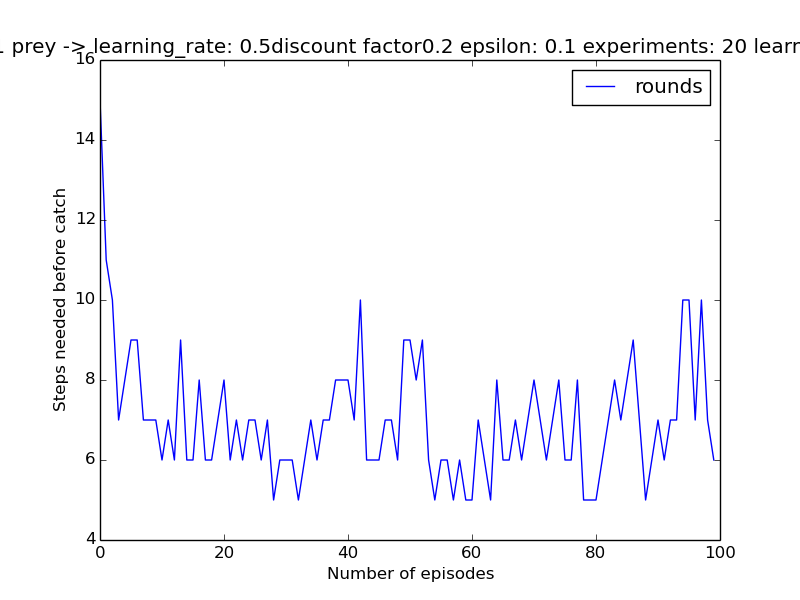
\includegraphics[scale=0.3]{minimax_100rounds_20exp_disc02_alpha05}
	\captionof{figure}{Minimax-Q: 1 predator versus 1 prey, with discount factor of 0.2}
	\label{graph:1vs1_disc_02}
\end{center}

\begin{center}
	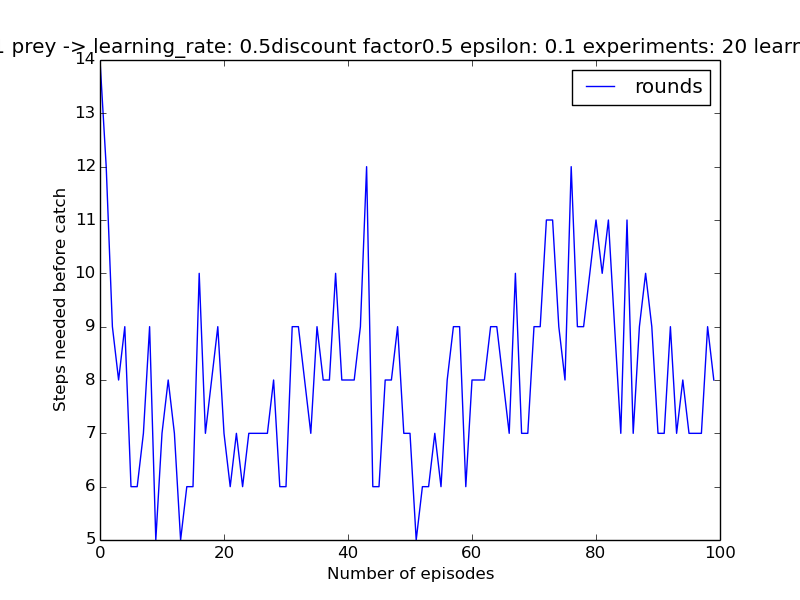
\includegraphics[scale=0.3]{minimax_100rounds_20exp_disc05_alpha05}
	\captionof{figure}{Minimax-Q: 1 predator versus 1 prey, with discount factor of 0.5}
	\label{graph:1vs1_disc_05}
\end{center}

\begin{center}
	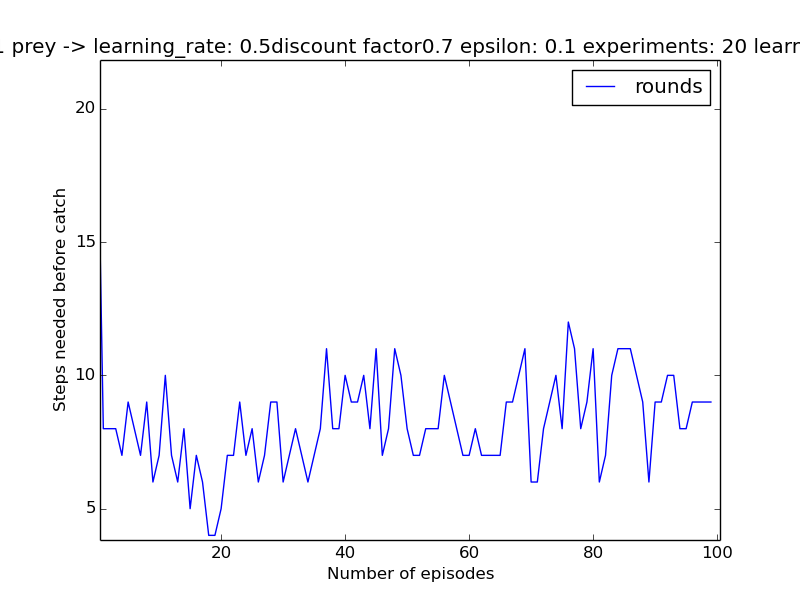
\includegraphics[scale=0.3]{minimax_100rounds_20exp_disc07_alpha05}
	\captionof{figure}{Minimax-Q: 1 predator versus 1 prey, with discount factor of 0.7}
	\label{graph:1vs1_disc_07}
\end{center}

Though the results seem very noisy, it is clear that a low discount factor yields best results. Again, this is essential to ensure that the predators do not collide. As you can see in Figure \ref{graph:1vs1_disc_02_50exp} where more experiments are run ,the graph shows a smoother line and you can see the agent learns to catch the prey. The number of steps to catch the prey converges to somewhere between 4 and 8.  

\begin{center}
	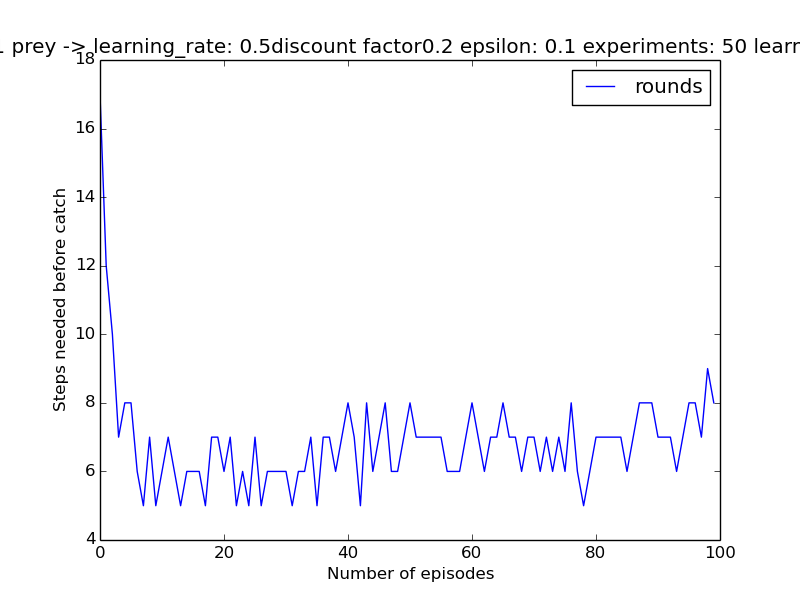
\includegraphics[scale=0.3]{minimax_gridsize5_100round_50exp_disc02_learningrate_05}
	\captionof{figure}{Minimax-Q: 1 predator versus 1 prey, with discount factor of 0.2}
	\label{graph:1vs1_disc_02_50exp}
\end{center}

In comparison with the Q-learning algorithm for the same parameters (Figure \ref{graph:Q1vs1_disc_02_50exp}) Minimax-Q (Figure  \ref{graph:1vs1_disc_02_50exp}) has a better performance. The average steps taken for the first 50 rounds are around 60 steps, while the Minimax-Q already has an average of 6 steps. This is due to the fact that Minimax-Q takes into account the prey's action that is worst for the predator and uses this to update it's policy and Q-values.

\begin{center}
	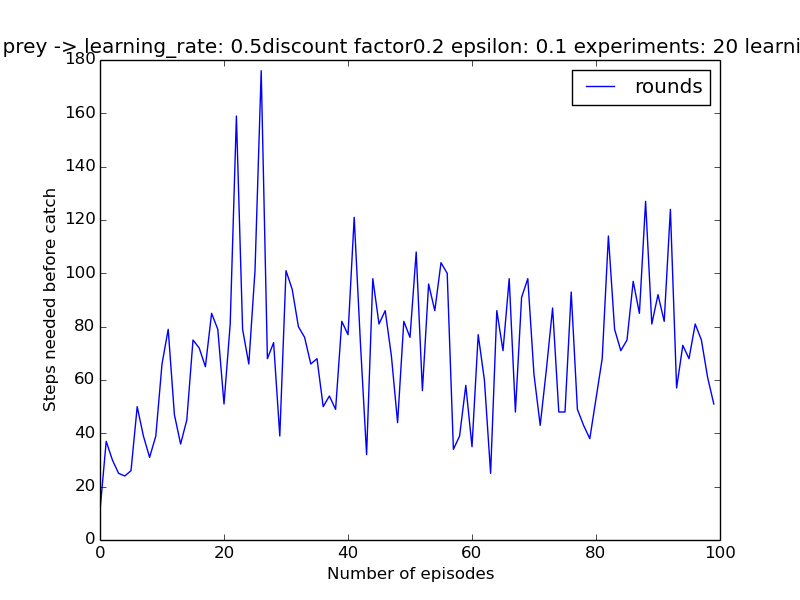
\includegraphics[scale=0.3]{qlearning_100rounds_20exp_disc02_alpha05}
	\captionof{figure}{Q-learning: 1 predator versus 1 prey, with discount factor of 0.2}
	\label{graph:Q1vs1_disc_02_50exp}
\end{center}
